

\documentclass[a4paper,12pt]{article}
\voffset=-1.5cm
\oddsidemargin=0.0cm
\textwidth = 480pt
\usepackage{eurosym}
\usepackage{vmargin}
\usepackage{amsmath}
\usepackage{graphics}
\usepackage{epsfig}
\usepackage{subfigure}
\usepackage{fancyhdr}
%\usepackage{listings}
\usepackage{amsmath}
\usepackage{graphicx}
\usepackage{amssymb}
\usepackage{framed}
\usepackage{multicol}
%=====================================================%
\usepackage{enumerate}
\usepackage{framed}
\usepackage{graphicx}
\usepackage{amsmath}
\usepackage{chngpage}
%\usepackage{bigints}


\setcounter{MaxMatrixCols}{10}
%TCIDATA{OutputFilter=LATEX.DLL}
%TCIDATA{Version=5.00.0.2570}
%TCIDATA{<META NAME="SaveForMode" CONTENT="1">}
%TCIDATA{LastRevised=Wednesday, February 23, 2011 13:24:34}
%TCIDATA{<META NAME="GraphicsSave" CONTENT="32">}
%TCIDATA{Language=American English}
\begin{document}
\subsection*{Question 1 - Short Questions}
\begin{enumerate}[(i)]
	%Unit 5 - Review Question 11
	%Page 112
	\item (4 marks) What is meant by the sampling distribution of the mean? Provide a hypothetical example in your explanation.\\
	\textbf{Need to show the two formulas for the mean and the standard deviation and
		some explanation about it being the mean of the distribution of means.}
	
	\item (4 marks) What is a trimmed mean? In what circumstances would you use this measure in preference to the arithmetic mean?\\
	\textbf{Removing a percentage of the data items from each end of the distribution and
		then re calculating the mean. Can be used to see the effect of outliers}
	\item (4 marks) What information does a 95\% confidence interval for the mean give us? \\
	\textbf{In repeated sampling you are confident that the true mean will be contained in
		that interval 95\% of the time}
	%=============================================%
	%Unit 6 - Review Question 18 and 19
	%Page 144
	\item (4 marks) What is a Type I error and a Type II error?\\
	\textbf{Type I error:\\
		When the null hypothesis is true and you reject it, you make a type I error. The probability of making a type I error is $\alpha$, which is the level of significance you set for your hypothesis test. }\\
	\textbf{Type II error:\\
		When the null hypothesis is false and you fail to reject it, you make a type II error. The probability of making a type II error is $\beta$, which depends on the power of the test. }
	%=============================================%
	%Unit 7 - Review Question 2
	%Page 166
	\item (4 marks) What are the tests that you can perform when comparing two populations?\\
	\textbf{Discussion of material on any two of the three tests from Unit 7.4. 2 Marks per Test}
	%=============================================%
	%Unit 8 - Review Question 7
	%Page 189
	
	\item (4 marks) What are the key components that need to be identified when designing an
	experiment?
	\textbf{The following are the components of an experimental design:
	(1) An experimental unit is an individual object from the sample from
		which you obtained some measurement.
	(2) A factor is some variable whose value is controlled by the experimenter.
	(3) A level is the intensity setting of a factor.
	(4) A treatment is a combination of factor levels.
	(5) A response is the variable being measured by the experimenter.}\\
(\textit{1 Mark for any 4})
	%=============================================%
	%Unit 8 - Review Question 7
	%Page 189
	
	\item (4 marks) What distinguishes a factorial experiment from a completely randomised
	experiment or a randomised block experiment?
	
	\textbf{ If there is interaction, then the other source of variation becomes a factor and
		possible interaction between factors must be included in the experimental
		design. The type of design that allows for interaction is an a x b Factorial
		Experiment. This design is classified as two-way.}
	
	%=============================================%
	%Unit 9 - Review Question 4
	%Page 216
	
	\item (4 marks) What is the difference between a ``between treatments" estimate and a ``within
	treatments" estimate?
	
	\textbf{Between treatments; variability among sample means. within treatment;
		variability of the data within the sample.}
	%=============================================%
	
	%Unit 10 - Review Question 1
	%Page 244
	
	\item  (4 marks) What is meant by multicollinearity? Describe some of the indicators of multicollinearity.
	
	\textbf{Multicollinearity may occur if there is a significant correlation between 2 or more of
		the independent variables. It often explains why a model that appears to make sense
		does not produce the desired results. }\\
	\textbf{The following are indicators that your regression
		model is likely to exhibit multicollinearity during your analysis:
		The value of the R-sq is large indicating a good fit, but the individual t-tests are
		not significant.}\\
	\textbf{The signs of the regression coefficients are not what you would have expected
		them to be; that is, contributing negatively rather than positively.
		A matrix of correlations generated by Minitab shows that some of the
		independent (predictor) variables are highly correlated.}
	
	%=============================================%
	%Unit 10 - Review Question 2
	%Page 244
	
	\item (4 marks) How does stepwise regression work and why would you use it?\\
	\textbf{Stepwise Regression is a variable selection procedure, provided as a built-in function in Minitab and it fits a variety of models
		to the data, adding and deleting variables based on their significance in relation to
		other variables in the model. It does this over a number of iterations until all significant
		variables have been added to the model. }
	%=============================================%
	\item (4 marks) In the context of analyzing categorical data, what is a Goodness of Fit test?\\ 
	\textbf{The goodness of fit test is based
		on comparing the observed results with the expected results, to see if there is any significant difference.
		The expected results are the results you would expect to see if the null
		hypothesis were true.}
	%=============================================%
	\item (4 marks) State the purpose of the Mann-Whitney U Test and the Kruskall Wallis Test. Include in your answer comparisons to the parametric counterpart to these tests.\\
	\textbf{The Mann Whitney U test is an alternative to the independent 2-sample t test and does
	not rely on normality or homogeneity of variance assumptions. The test is based on the
	ranking of data. It is as powerful as the t test.}\\
	\textbf{The non-parametric equivalent of the F test is the Kruskal-Wallis test.
	This test is also based on ranking the data. It uses the chi-squared
	statistic rather than the F test to calculate probabilities. The null and
	alternative hypotheses are the same as for the ANOVA.}
	%=============================================%
	
\end{enumerate}

\subsection*{Question 2 - Exeprimental Design}


\subsubsection*{Part A}
\begin{itemize}
	\item The student must demonstrate a level of understanding.
	\item  It is not enough to just state
	the P value. The argument must follow the correct steps as set out and both p value
	and confidence interval should be referred to as evidence.
	\item Definite statement of Null and Alternative Hypothesis for both tests
	\item Risk Criteria
	\item Decision Criteria
	\item Conclusion
\end{itemize}
\subsubsection*{Part B}
\begin{itemize}
	\item The student must demonstrate a level of understanding.
	\item  It is not enough to just state
	the P value. The argument must follow the correct steps as set out and both p value
	and confidence interval should be referred to as evidence.
	\item Definite statement of Null and Alternative Hypothesis for both tests
	\item Risk Criteria
	\item Decision Criteria
	\item Conclusion
\end{itemize}

\newpage
\subsection*{Question 3 - Normal Distribution}
\subsubsection*{Part A}

\noindent Marking Scheme:
\begin{itemize}
	\item 4 Marks for showing the relevant calculations,
	\item 1 Mark for drawing the boxplots to a satisfactory standard.
	\item 1 Mark for a well-explained conclusion,
\end{itemize}



\subsubsection*{Part B}
Variable X : Not Normally Dsitributed
\begin{itemize}
	\item Histogram doesnt align well with density curve. Density curve is centred.
	\item QQ plot : Dots dont follow the trend line
	\item Boxplot is not symmetric
	\item Anderson Darling Test has significant result
	%	\item Median and Mean are not similar
\end{itemize}
Variable X :  Normally Dsitributed
\begin{itemize}
	\item Histogram align reasonable well with density curve. Density curve is centred.
	\item QQ plot : Dots mostly follow the trend line
	\item Boxplot is symmetric
	\item Anderson Darling Test does not have significant result
	%	\item Median and Mean are not similar
\end{itemize}

\subsubsection*{Part C}
\noindent \textbf{Part 1}
\begin{itemize}
	
	\item Z score
	\[  z = \frac{x-\mu}{\sigma} = \frac{1004.1-1002.5}{1.25} = \frac{1.6}{1.25} = 1.28\]
	
	\item Using Murdoch Barnes Tables
	\[ P(Z \geq 1.29) = 0.1003\]
	
	\item Answer: $P(X \geq 1004.1) =0.1003$
	
\end{itemize}
\begin{figure}[h!]
	\centering
	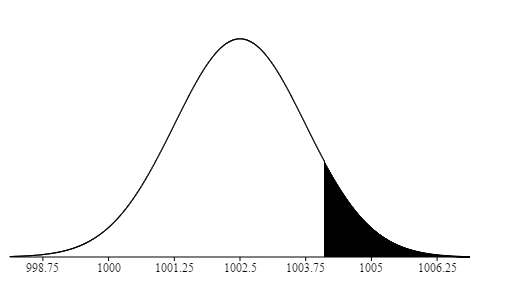
\includegraphics[width=0.35\linewidth]{images/Parts1004}
	
\end{figure}
\newpage
\noindent \textbf{Part 2}
\begin{itemize}
	
	\item Z score
	\[  z = \frac{x-\mu}{\sigma} = \frac{1000-1002.5}{1.25} = \frac{-2.5}{1.25} = -2\]
	
	\item Symmetry Rule
	\[ P(Z \leq -2) = P(Z \geq 2) \]
	\item Using Murdoch Barnes Tables
	\[ P(Z \geq 2) = 0.02275\]
	
	\item Answer: $P(X \leq 1000) =0.00275$
	
\end{itemize}
\begin{figure}[h!]
	\centering
	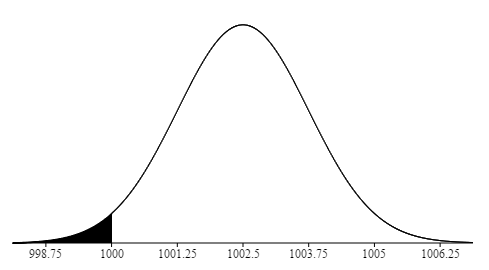
\includegraphics[width=0.35\linewidth]{images/Parts1000}
	
\end{figure}
\noindent \textbf{Part 3}

\begin{itemize}
	
	\item Z score
	\[  z = \frac{x-\mu}{\sigma} = \frac{1005-1002.5}{1.25} = \frac{2.5}{1.25} = 2\]
	
	
	\item Using Murdoch Barnes Tables
	\[ P(Z \geq 2) = 0.02275\]
	
	
	\item From Before $P(X \leq 1000) =0.00275$
	\item Probability of being outside the interval 
	\[P(X \leq 1000) + P(X \leq 1000)  = 2 \times 0.02275 \approx 0.0455\]
	\item If 99\% within interval, then only 1\% outside interval
	\item Therefore we conclude that the Claim is false
\end{itemize}


\begin{figure}[h!]
	\centering
	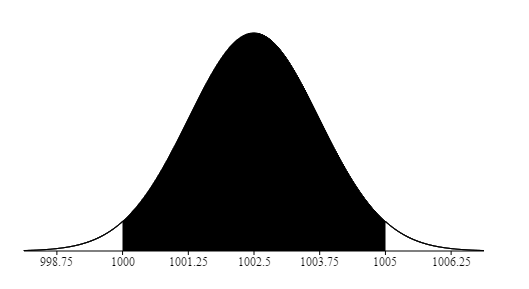
\includegraphics[width=0.35\linewidth]{images/between1000and1005}
	
\end{figure}


\newpage
%==============================================================================%




\subsection*{Question 4}
\subsubsection*{Part A - Two Sample Test}
\textit{Suppose a company manufactures a particular product in two facilities: Factory A and Factory B.
The management wants to make sure that the Factory B, which has been recently constructed, is manufacturing 
components to the same specifications as Factory A.}
\\
\noindent \textit{Measurement data from both factories has been compiled and analysed, with the following Minitab output has been created.}

\noindent \textbf{Key Conclusions}
\begin{itemize}
	\item Significant Difference in Means
	\item Significant Difference in Variances
	\item Processes in both factories not working to same specification
	\item Equipment in Factory B needs to be re-calibrated.
\end{itemize}

\subsubsection*{Part B - Chi Square}



\begin{itemize}
	\item[1.] Evidence that demonstrates a clear
	understanding of the test and its outcomes. 
	\item[2.] Expected Values
	\[  \frac{\mbox{Row Total} \times \mbox{Grand Total} }{\mbox{Grand Total}} \]
	\item[3.] Degrees of Freedom = 4 i.e. (r-1) x (c-1)
	
	\item[4.]  Good interpretation of the data from the table combined with the correct
	statistical analysis.  Comment on the significance of a p value being less than 0.05. There is no association…..There is association.

\end{itemize}

%=====================================================================%
\newpage\subsection*{Question 5: Regression Analysis}
\subsubsection*{Part A - Simple Linear Regression Analysis}
\begin{itemize}
\item[1.] 3 marks for each correct value (4 for correct p-value) 

\[\frac{1.016}{0.790} = 1.29\]
\[\frac{x}{0.790} = 5.61 \therefore x = 0.3640\]
\item[2.] Statement and Interpretation of the regression line
\[Tensile = 1.016 + 0.364 Knots\]
 
\item[3.] Noting the relationship was significant
\item[4.] \[Tensile = 1.016 + 0.364 \times 10\]
\item[5.] Stating and interpreting the R squared value 
\end{itemize}

	
%===========================================%
\subsubsection*{Part B - Residuals}
 Minitab can provide four diagnostic plots to help you appraise the quality of a linear model.	What is the purpose of the diagnostic plots and what does each one tell you?\\ 
 \bigskip

\noindent	\textbf{Checking for Normality of Residuals $\times 2$, Heteroscedascity, Autocorrelation}
%===========================================%
\subsubsection*{Part C - MLR}
\begin{itemize}
\item Short Discussion / Interpretation of the regression line
\item Noting the significant and non significant relationships 
\item Stating and interpreting the R squared value 
\item A discussion about the possibility of the presence of multicolinearity and the possible
use of stepwise regression to eliminate it 

\end{itemize}

\end{document}